% ============================================================
%  Příprava na maturitu – Elektrotechnika
%  Okruh 9: Energetická rozvodná soustava a kvalita el. energie
% ============================================================

\documentclass[a4paper,10pt]{article}

\usepackage[T1]{fontenc}
\usepackage[utf8]{inputenc}
\usepackage[left=2.0cm, right=1.8cm, top=1.8cm, bottom=1.8cm]{geometry}
\usepackage{parskip}
\usepackage{xcolor}
\usepackage{tabularx}
\usepackage{booktabs}
\usepackage{tikz}
\usepackage{mdframed}
\usepackage{amsmath}
\usepackage{enumitem}
\usepackage{circuitikz}

\usetikzlibrary{arrows.meta, positioning, decorations.pathmorphing, shapes.geometric, calc}

% --- Barvy ---
\definecolor{accent}{HTML}{1A3A5C}
\definecolor{lightblue}{HTML}{EAF2F8}
\definecolor{lightyellow}{HTML}{FDFBE4}
\definecolor{lightgreen}{HTML}{EAF7EA}
\definecolor{lightred}{HTML}{FDE8E8}
\definecolor{lightgray}{HTML}{F4F4F4}

% --- Boxy ---
\newmdenv[backgroundcolor=lightblue,linecolor=accent!40,roundcorner=4pt,
  innertopmargin=6pt,innerbottommargin=6pt,innerleftmargin=8pt,innerrightmargin=8pt]{pojmybox}
\newmdenv[backgroundcolor=lightyellow,linecolor=accent!30,roundcorner=4pt,
  innertopmargin=6pt,innerbottommargin=6pt,innerleftmargin=8pt,innerrightmargin=8pt]{vysvetlenibox}
\newmdenv[backgroundcolor=lightgreen,linecolor=accent!40,roundcorner=4pt,
  innertopmargin=6pt,innerbottommargin=6pt,innerleftmargin=8pt,innerrightmargin=8pt]{vzorcebox}
\newmdenv[backgroundcolor=lightred,linecolor=accent!30,roundcorner=4pt,
  innertopmargin=6pt,innerbottommargin=6pt,innerleftmargin=8pt,innerrightmargin=8pt]{durazbox}

\setlist[itemize]{noitemsep, leftmargin=1.4em, topsep=2pt}
\setlist[enumerate]{noitemsep, leftmargin=1.4em, topsep=2pt}

% --- Zkratka pro jednotky ---
\newcommand{\jednotka}[1]{\,[\mathrm{#1}]}

\begin{document}

% ============================================================
\section*{\large Okruh 9 – Energetická rozvodná soustava a kvalita el. energie}

\begin{pojmybox}
\textbf{Klíčové pojmy:}
elektroenergetická soustava (ES), přenosová soustava, distribuční soustava, napěťové hladiny (NN, VN, VVN, ZVN), zapojení hvězda/trojúhelník, fázové a sdružené napětí, topologie sítě, kvalita elektrické energie (harmonické, flikr, nesymetrie)
\end{pojmybox}

\begin{vysvetlenibox}

% ================================================================
\subsection*{1. Struktura elektroenergetické soustavy (ES)}

ES je propojený soubor zařízení pro výrobu, přenos, transformaci a distribuci elektřiny. Jejím cílem je zajistit spolehlivou dodávku energie.

\textbf{Hladiny napětí v ČR:}
\begin{itemize}
    \item \textbf{ZVN (Zvláště vysoké napětí):} 400 kV – Páteřní přenosová soustava (ČEPS), mezinárodní propojení.
    \item \textbf{VVN (Velmi vysoké napětí):} 110 kV – Regionální přenos, napojení velkých rozvoden a průmyslu.
    \item \textbf{VN (Vysoké napětí):} 22 kV (v městech někdy 10 kV nebo 35 kV) – Primární distribuce k obecním trafo-stanicím.
    \item \textbf{NN (Nízké napětí):} 400 / 230 V – Koncová distribuce k domácnostem.
\end{itemize}

\begin{center}
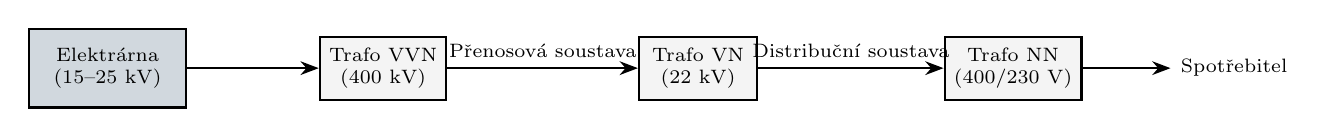
\begin{tikzpicture}[>=Stealth, font=\scriptsize, thick]
  % Bloky s přidaným align=center
  \node[draw, fill=accent!20, minimum width=2cm, minimum height=1cm, align=center] (gen) at (0,0) {Elektrárna\\(15--25 kV)};
  \node[draw, fill=lightgray, minimum width=1.5cm, minimum height=0.8cm, align=center] (t1) at (3.5,0) {Trafo VVN\\(400 kV)};
  \node[draw, fill=lightgray, minimum width=1.5cm, minimum height=0.8cm, align=center] (t2) at (7.5,0) {Trafo VN\\(22 kV)};
  \node[draw, fill=lightgray, minimum width=1.5cm, minimum height=0.8cm, align=center] (t3) at (11.5,0) {Trafo NN\\(400/230 V)};

  % Propojení
  \draw[->] (gen) -- (t1);
  \draw[->] (t1) -- (t2) node[midway, above] {Přenosová soustava};
  \draw[->] (t2) -- (t3) node[midway, above] {Distribuční soustava};
  \draw[->] (t3) -- (13.5,0) node[right] {Spotřebitel};
\end{tikzpicture}
\end{center}

% ================================================================
\subsection*{2. Trojfázová soustava a napětí}

V rozvodné soustavě používáme tři fáze (L1, L2, L3) posunuté o $120^\circ$.

\textbf{Typy napětí v síti NN:}
\begin{itemize}
    \item \textbf{Fázové napětí ($U_f$):} Napětí mezi fází a nulovým vodičem (N). V ČR $U_f = 230\,\mathrm{V}$.
    \item \textbf{Sdružené napětí ($U_s$):} Napětí mezi dvěma fázemi. V ČR $U_s = 400\,\mathrm{V}$.
\end{itemize}

\begin{vzorcebox}
\[
U_s = \sqrt{3} \cdot U_f \quad \implies \quad 230 \cdot 1{,}732 \approx 400\,\mathrm{V}
\]
\end{vzorcebox}

\textbf{Způsoby zapojení:}
\begin{enumerate}
    \item \textbf{Hvězda (Y):} Má společný uzel (střed), ze kterého se vyvádí nulový vodič (N). Používá se pro napájení domácností (máme k dispozici 230V i 400V).
    \item \textbf{Trojúhelník (D):} Nemá střední bod. Používá se pro přenos VN/VVN a pro průmyslové motory.
\end{enumerate}

\begin{center}
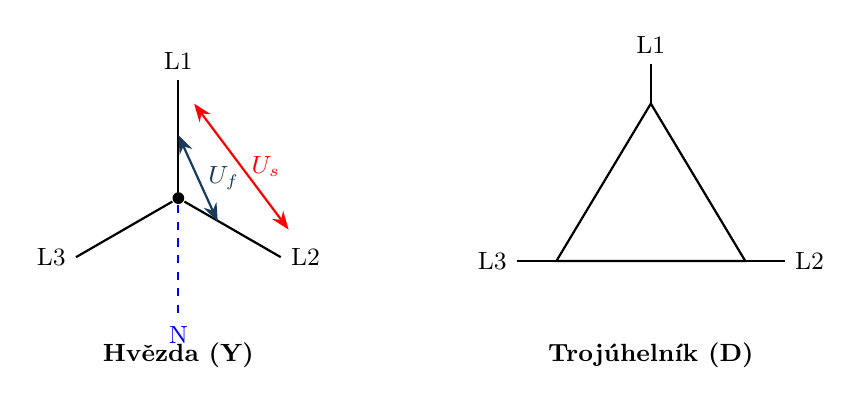
\begin{tikzpicture}[>=Stealth, font=\small, thick]
  % Hvězda
  \begin{scope}[xshift=0cm]
    \draw (0,0) node[circle, fill, inner sep=1.5pt] (N) {} -- (0,1.5) node[above] {L1};
    \draw (N) -- (-1.3,-0.75) node[left] {L3};
    \draw (N) -- (1.3,-0.75) node[right] {L2};
    \draw[blue, dashed] (N) -- (0,-1.5) node[below] {N};
    \node at (0, -2) {\textbf{Hvězda (Y)}};
    \draw[<->, accent] (0,0.8) -- (0.5, -0.3) node[midway, right] {$U_f$};
    \draw[<->, red] (0.2,1.2) -- (1.4, -0.4) node[midway, right] {$U_s$};
  \end{scope}

  % Trojúhelník
  \begin{scope}[xshift=6cm]
    \draw (0,1.2) -- (1.2,-0.8) -- (-1.2,-0.8) -- cycle;
    \draw (0,1.2) -- (0,1.7) node[above] {L1};
    \draw (1.2,-0.8) -- (1.7,-0.8) node[right] {L2};
    \draw (-1.2,-0.8) -- (-1.7,-0.8) node[left] {L3};
    \node at (0, -2) {\textbf{Trojúhelník (D)}};
  \end{scope}
\end{tikzpicture}
\end{center}

% ================================================================
\subsection*{3. Topologie distribučních sítí}

Způsob, jakým jsou propojeny stanice a spotřebitelé:
\begin{itemize}
    \item \textbf{Paprsková (radiální):} Jednoduchá, nejlevnější. Při poruše na začátku je celá větev bez proudu. (Sítě NN na vesnicích).
    \item \textbf{Okružní:} Vedení tvoří smyčku, která začíná a končí v jednom bodě. Při poruše lze místo odpojit a napájet z druhé strany. (Typické pro VN v městech).
    \item \textbf{Mřížová:} Velmi spolehlivá, napájení z více stran. Nejdražší. (Centra velkoměst).
\end{itemize}

% ================================================================
\subsection*{4. Kvalita elektrické energie (ČSN EN 50160)}

Elektrická energie je považována za zboží a musí splňovat určité parametry. Pokud nejsou splněny, může dojít k poškození citlivých přístrojů nebo přehřívání motorů a transformátorů.

\textbf{Hlavní sledované parametry:}
\begin{enumerate}
    \item \textbf{Frekvence:} $50\,\mathrm{Hz} \pm 1\,\%$. Kolísá při nerovnováze mezi výrobou a spotřebou (\textit{viz Okruh 8}).
    \item \textbf{Velikost napětí:} Dovolená odchylka je $\pm 10\,\%$ ($207\,\mathrm{V} \text{ až } 253\,\mathrm{V}$).
    \item \textbf{Harmonické zkreslení (THD):} Deformace sinusovky způsobená nelineárními spotřebiči (spínané zdroje PC, LED žárovky, frekvenční měniče). Způsobují ztráty a rušení.
    \item \textbf{Nesymetrie:} Rozdílné zatížení jednotlivých fází (L1, L2, L3), což vede k proudům v nulovém vodiči.
    \item \textbf{Flikr (Míhání):} Kolísání napětí způsobující nepříjemné blikání světel (např. vlivem provozu elektrických obloukových pecí nebo kolísání větru u VTE).
\end{enumerate}

\begin{durazbox}
\textbf{Zkrat a přetížení v soustavě:}
\begin{itemize}
    \item \textbf{Zkrat:} Vodivé spojení fází nebo fáze se zemí. Proud je limitován pouze impedancí sítě, dosahuje kA. Musí být ihned odpojen jističem (\textit{viz Okruh 5}).
    \item \textbf{Přetížení:} Odběr většího výkonu, než na který je síť dimenzována. Způsobuje přehřívání vodičů a pokles napětí.
\end{itemize}
\end{durazbox}

% ================================================================
\subsection*{5. Kompenzace v rozvodné síti}

Jak jsme probrali v \textbf{Okruhu 4}, jalový výkon zatěžuje vedení. Rozvodné závody (distribuce) vyžadují od velkoodběratelů, aby udržovali účiník $\cos \varphi$ v rozmezí \textbf{0,95 až 1}. Pokud odebírají příliš mnoho jaloviny, platí vysoké pokuty, protože tato energie zbytečně zahřívá dráty a transformátory soustavy.

% ================================================================
\subsection*{6. Shrnutí – parametry sítě NN}

\begin{center}
\begin{tabularx}{0.97\linewidth}{@{} l l X @{}}
\toprule
\textbf{Veličina} & \textbf{Hodnota} & \textbf{Poznámka} \\
\midrule
Jmenovitá frekvence & $50\,\mathrm{Hz}$ & Stabilita výroby vs. spotřeby \\
Fázové napětí $U_f$ & $230\,\mathrm{V}$ & Proti vodiči N \\
Sdružené napětí $U_s$ & $400\,\mathrm{V}$ & Mezi fázemi (L1-L2, \ldots) \\
Tolerance napětí & $\pm 10\,\%$ & Norma ČSN EN 50160 \\
Sled fází & L1, L2, L3 & Důležité pro směr otáčení motorů \\
\bottomrule
\end{tabularx}
\end{center}

\end{vysvetlenibox}

\end{document}
